The design approach described in this article is not intended to
replace sound engineering of an intelligent system, but rather as
an additional step that may be applied in order to provide
the system with more agility, flexibility, and the ability to be rapidly
re-tasked. This is accomplished by assuring that the appropriate knowledge
of the correct scope and format is available to all modules of the
intelligent system.

\begin{figure}[ht!]
\begin{center}
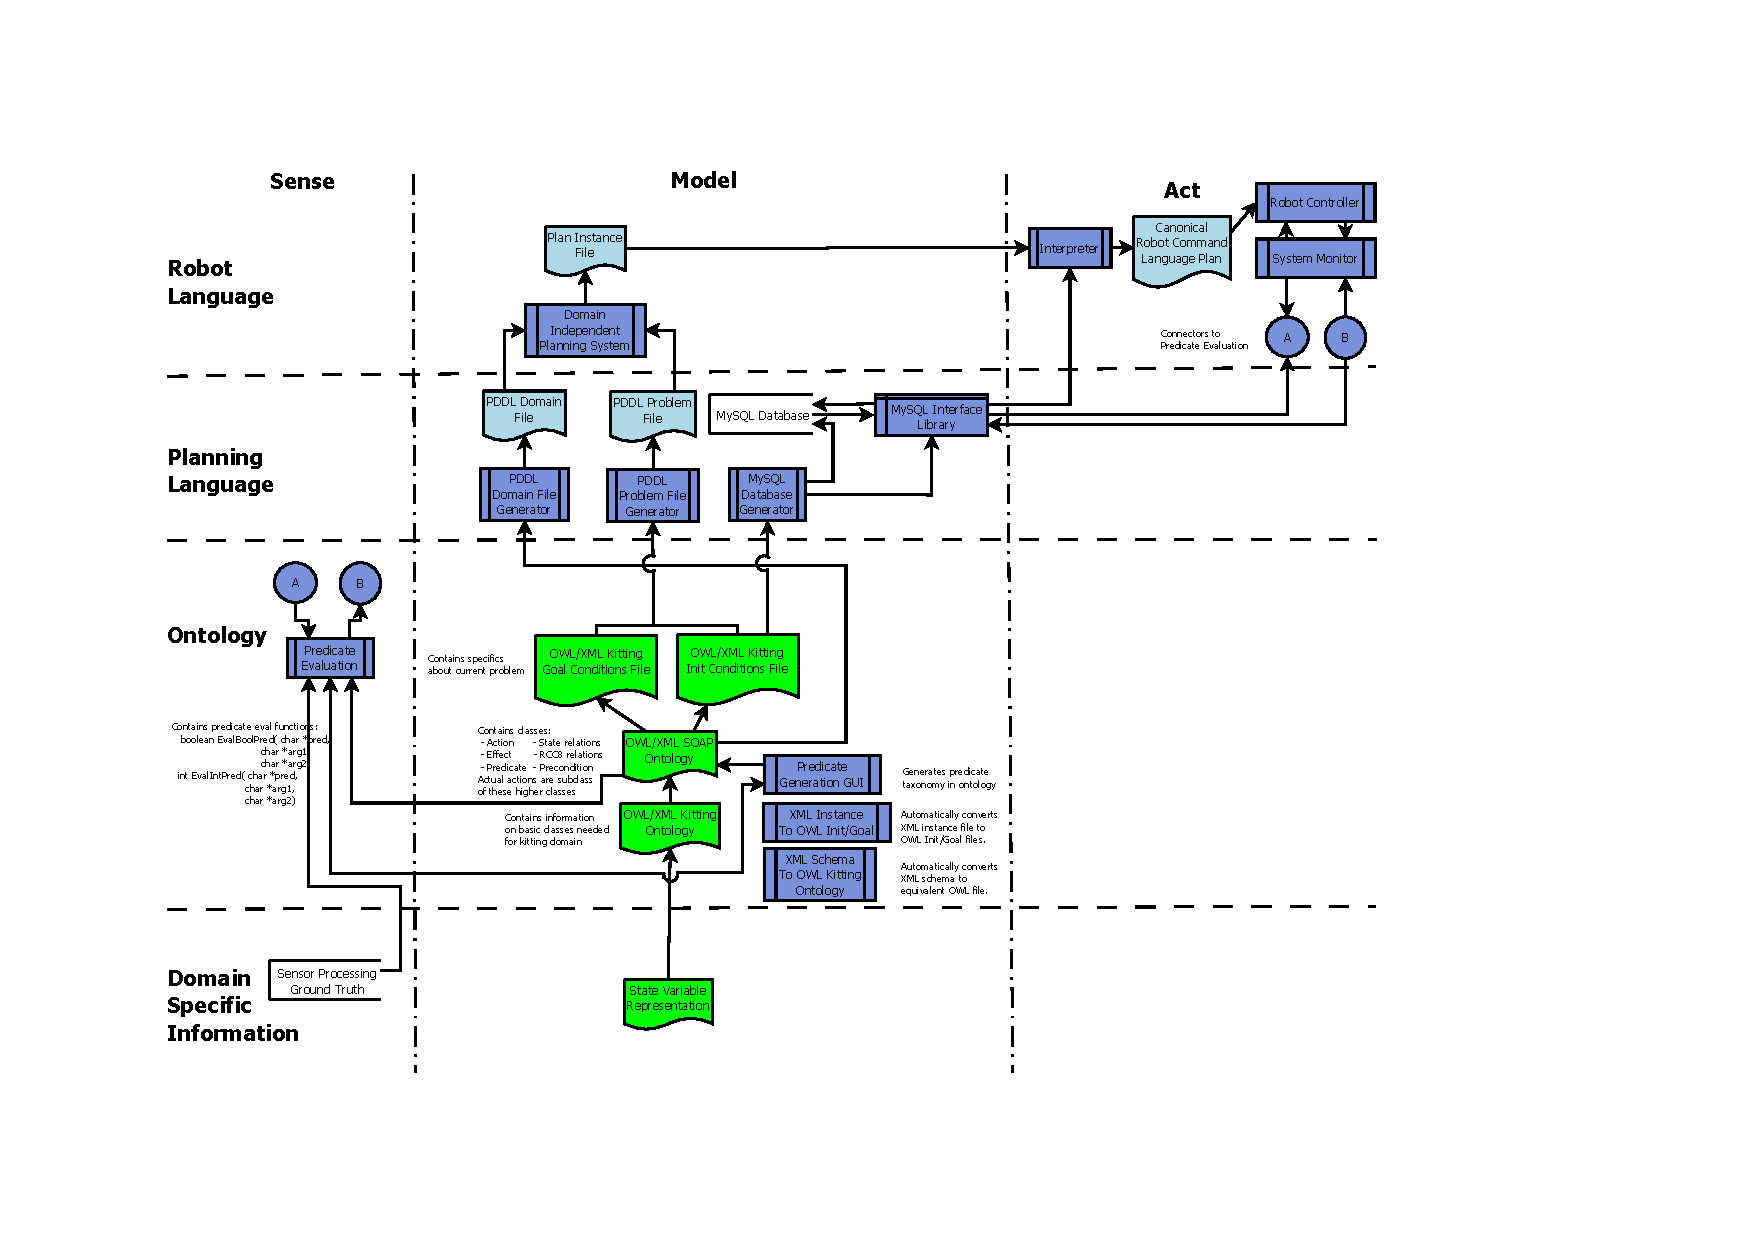
\includegraphics[width=13cm]{images/KnowledgeDrivenRobotics.pdf}
\caption{Knowledge Driven Design extensions -- In this figure, green shaded boxes with curved bottoms
represent hand generated files while
light blue shaded boxes with curved bottoms represent automatically created boxes. Square
boxes represent processes and libraries.}
\label{fig:DesignArchitecture}
\end{center}
\end{figure}

The overall knowledge model of the system may be seen in Figure \ref{fig:DesignArchitecture}.
The figure is organized vertically by the representation that is used for the knowledge
and horizontally by the classical sense-model-act paradigm of intelligent systems.
On the vertical axis, knowledge begins with Domain Specific Information that captures
operational knowledge that is necessary to be successful in the particular domain in which
the system is designed to operate. This information is then organized into a domain
independent representation (an Ontology) that allows for the encoding of an object
taxonomy, object-to-object
relationships, and aspects of actions, preconditions, and effects.
Aspects of this
knowledge are automatically extracted and encoded in a form that is optimized for
a planning system to utilize (the Planning Language). Once a plan has been formulated,
the knowledge is transformed into a representation that is optimized for use by a robotic system
(the Robot Language).

It is acknowledged that sensing and action are important parts of a robotic system.
However, this article focuses on knowledge representation, and thus the modeling section
will be described in the most detail.

\subsection{Domain Specific Information}
The most basic knowledge that must be gathered for a knowledge
driven system is domain specific information (DSI). This appears along the bottom row of
Figure \ref{fig:DesignArchitecture}. DSI includes sensors and sensor processing that
are specifically tuned to operate in the target domain. Examples of sensor processing
may include pose determination and object identification.

For the knowledge model, a scenario driven approach is taken where
the DSI design begins with a domain expert creating one or more use cases and specific
scenarios that describe the typical operation of the system. Based on these scenarios and
use cases, the high-level
actions that the system must be able to accomplish can be enumerated and described.
An action description that includes any preconditions that
must be true for an action to be valid as well as expected effects that will result from a
given action is then created for each action.

\begin{figure}[ht!]
\centering
\textsl{put-kittray}($\mathit{robot}$,$\mathit{kittray}$,$\mathit{worktable}$): The \textit{Robot}
$\mathit{robot}$ puts the \textit{KitTray} $\mathit{kittray}$ on the \textit{WorkTable} $\mathit{worktable}$.

\begin{tabular}{ l|l }
  \textit{preconditions} & \textit{effects} \\
  \hline
  \small {\textsf{kittray-location-robot}}(\small $\mathit{kittray}$,\small $\mathit{robot}$)
  &$\neg$\small {\textsf{kittray-location-robot}}(\small $\mathit{kittray}$,\small $\mathit{robot}$)\\
  \small {\textsf{robot-holds-kittray}}(\small $\mathit{robot}$,\small $\mathit{kittray}$)
  &$\neg$\small {\textsf{robot-holds-kittray}}(\small $\mathit{robot}$,\small $\mathit{kittray}$)\\
  \small {\textsf{worktable-empty}}(\small $\mathit{worktable}$)
  &$\neg$\small {\textsf{worktable-empty}}(\small $\mathit{worktable}$)\\
  &\small {\textsf{kittray-location-worktable}}(\small $\mathit{kittray}$,\small $\mathit{worktable}$)\\
  &\small {\textsf{robot-empty}}(\small $\mathit{robot}$)\\
  &\small {\textsf{on-worktable-kittray}}(\small $\mathit{worktable}$,\small $\mathit{kittray}$)\\
\end{tabular}
\caption{Example action along with its preconditions and expected effects.}
\label{fig:ActionExample}
\end{figure}

Based on the action description, objects in the environment that are relevant
for system operation can be identified. For example, the action depicted in Figure \ref{fig:ActionExample}
has a given robot place a kit tray onto a work table. The preconditions for this action are that
the robot is holding a kit tray and there is a clear space on the table to place the tray. This is
represented by the predicate expressions shown in Figure \ref{fig:ActionExample} that specify that
the robot is holding the kit tray, the kit tray is located on the robot (actually in its gripper), and
the work table is empty. The expected effects of this action are that the kit tray is now located
on the work table and the robot is no longer holding it. This is also represented by a series
of predicates that are shown in Figure \ref{fig:ActionExample}. Based on the preconditions and expected effects,
the objects that are relevant to this action include the robot, the kit tray, and the work table.
Aspects of these items may now be represented in the DSI. For example, that a kit tray has a location and may
be held by the robot or placed on the work table.

\subsection{Ontology}
The design transitions from domain expertise to knowledge modeling expertise
when the State Variable Representation (SVR) is used to generate an ontology which consists of three parts:
\begin{enumerate}
 \item A base ontology that describes the objects in the scenario. This file contains
all of the basic information that was determined to be needed during the evaluation of
the use cases and scenarios. The knowledge is represented in as compact of a form as
possible with knowledge classes inheriting common attributes from parent classes.
For example, the class for a work table, \class{WorkTable} is derived from
\class{BoxyObject}, and \class{BoxyObject} is derived from \class{SolidObject}. The actual size of the work table
is defined in the \class{BoxyObject}. The \class{WorkTable} includes all of the attributes
of a \class{BoxyObject} along with the notion that a work table is something that can have
other objects placed on it. The work table itself is part of a work station \class{WorkStation}.
 \item Extensions that describe the States of the world and relationships between states,
Ordering constructs, Actions, and Predicates (the \onto{SOAP} ontology)
that are relevant to the scenario. This extension contains not only the basic class for
actions and predicates, but also the individual actions and predicates that are necessary
for the domain under study. In the case of the kit building domain, it was found that
10 actions and 16 predicates were necessary.
 \item Instance files that describe the initial and goal states for the system. The final set
of files for the ontology contain a description of the complete system starting or initial state and the
requirements on the goal state. The initial state file must contain a description of the environment that
is complete enough for a planning system to be able to create a valid sequence of actions that will achieve
the given goal state. For the kit building domain, this includes information such as the location of the
various end effectors that are available to the robot, the locations and contents of part supply bins, and
the location where finished kits should be placed. The goal state file only needs to contain information that
is relevant to the end goal of the system. For the case of building a kit, this may simply be that a complete
kit is located in a bin designed to hold completed kits.
\end{enumerate}
The ontology files are
described in more detail in Section \ref{Sect:Ontology}.

\subsection{Planning Language}
The Planning Domain Definition Language (PDDL) \cite{PDDL} is an attempt by the
domain independent planning community to formulate a standard language
for planning. A community of planning researchers has been producing
planning systems that comply with this formalism since the first International
Planning Competition held in 1998. This competition series continues today,
with the seventh competition being held in 2011. PDDL is constantly
adding extensions to the base language in order to represent more expressive
problem domains. The work represented in this article is based on PDDL Version 3.
By placing the knowledge in a PDDL representation, the use of an
entire family of open source planning systems is enabled.

The PDDL input format consists
of two files that specify the domain and the problem. As shown in Figure
\ref{fig:DesignArchitecture}, these files are automatically
generated from the ontology. The domain file represents actions along
with required preconditions and expected results. The problem file
represents the initial state of the system and the desired goal.

From these two files, a domain independent planning system such as
the forward-chaining partial-order planning system from Coles \textit{et. al}
\cite{Coles.ICAPS.2010} may be run to create a static plan file. This
plan file contains a sequence of actions that will transition the
system from the initial state to the goal state.
In order to maintain flexibility, it is desired that detailed information
that is subject to change should be ``late-bound'' to the plan.
In other words, specific information is acquired directly before that
information needs to be used by the system.
This allows for last minute changes in this information. For example,
the location of a kit tray on a work table may be different from run to run.
However, one would like to be able to use the same planning sequence for
constructing the kit independent of the tray's exact position.
To compensate for this lack of exact knowledge, the plans that are
generated by the PDDL planning system contain only high-level actions.
\begin{figure}[t!h!]
\begin{minipage}{.5\paperwidth}
\begin{list}{}{\setlength{\leftmargin}{1em}}\item\small
\begin{Verbatim}[commandchars=\\\{\},fontsize=\scriptsize, numbers=left, numbersep=2pt]
(attach-endeffector robot_1 tray_gripper tray_gripper_holder changing_station_1)
(take-kittray robot_1 kit_tray_1 empty_kit_tray_supply tray_gripper work_table_1)
(put-kittray robot_1 kit_tray_1 work_table_1)
\ldots
(put-part robot_1 part_a_1 kit_a2b2c1 work_table_1 part_a_tray)
(remove-endeffector robot_1 part_gripper part_gripper_holder changing_station_1)
(attach-endeffector robot_1 tray_gripper tray_gripper_holder changing_station_1)
(take-kit robot_1 kit_a2b2c1 work_table_1 tray_gripper)
(put-kit robot_1 kit_a2b2c1 finished_kit_receiver)
\end{Verbatim}
\end{list}
\end{minipage}
\caption{Excerpt of the PDDL solution file for kitting.}
\label{fig:Solution}
\end{figure}

Figure \ref{fig:Solution} depicts an excerpt of a solution for
the construction of a kit. Line 3 with the command \textsl{put-kittray}
shows the command that is issued to place
a kit tray onto the work table. To facilitate late binding, this
command does not specify the exact location of the work table.
This kind of knowledge detail is maintained by sensor processing
and is stored in a MySQL database \cite{MySQL}. As shown
in Figure \ref{fig:DesignArchitecture}, the actual tables
for the database are auto-generated during the design phase and the
knowledge is utilized in combination with the PDDL planned action by
the interpreter in order to form Robot Language Commands.

\subsection{Robot Language}
While the high-level PDDL commands are a convenient representation
for the planning system, they do not contain the information that is
required by a robotic controller to successfully control a robotic cell.
The interpreter combines knowledge from the PDDL plan file with
knowledge from the MySQL database to form a sequence of sequential
actions that the robot controller is able to execute.
The authors devised a canonical robot
command language (CRCL) in which such lists can be written. The purpose of the
CRCL is to provide generic commands that
implement the functionality of typical industrial robots without being
specific either to the language of the planning system that makes a plan or
to the language used by a robot controller that executes a plan.

It was anticipated
that plans being generated by this system would
be executed by a variety of robot controllers using
robot-specific languages for input programs. The authors themselves are
using a ROS controller \cite{ROS} to control a
robot\footnote{Certain commercial/open source software and tools are identified
in this paper in order to explain our research. Such identification does not imply
recommendation or endorsement by the authors or NIST, nor does it
imply that the software tools identified are necessarily the best available for the purpose.}.
The controller and the interpreter are connected using files of robot commands in CRCL. After a plan
has been generated by the PDDL planner, the plan is translated into a CRCL
file. When the plan is being executed, the CRCL commands are translated
into ROS commands.

The CRCL includes commands for a robot controller. In normal system operation,
CRCL commands will be translated into the robot controller's native
language by the robot's plan interpreter as it works its way through a
CRCL plan. One CRCL command may be interpreted into several native
language commands.
One or more canonical robot commands may be placed on a queue and
executed (in order) when desired.
More information on CRCL commands may be found in
Balakirsky \textit{et. al} \cite{Balakirsky2012-1}.
